\documentclass{article}

\usepackage[xetex, colorlinks=true]{hyperref}
\usepackage[
   backend=biber,
   bibencoding=utf8,
   style=alphabetic,
   hyperref=true,
   % citestyle=authoryear-comp,
   backref=false,
   sortlocale=en,
   url=true, 
   doi=false,
   eprint=false
 ]{biblatex}
\addbibresource{biblio.bib}

\newcommand\Coq{Coq}
\newcommand\R{R}
\newcommand\Cn{C}

\usepackage{minted}
\setminted{encoding=utf8}

\usepackage{tikz}
\usetikzlibrary{positioning}

\tikzset{
	box/.style = {
		draw = black,
        fill = white,
		rectangle,
		rounded corners = 2pt,
		text centered,
		minimum height = 5mm,
		minimum width = 10mm
	}
}

\title{Notes about \R}
\author{Martin Bodin}

\begin{document}

\maketitle

\section{Presentation of the Language}

\R{} is now a trending programming language for mathematicians.
In practise, it is presented as a read-eval-print-loop,
but it is also possible to write programs in it.
The language enables easy integration of \Cn{} functions.

\subsection{History}

\R{} is a programming language designed for statistics.
Its specification~\parencite{team2000r} is not precise:
in practise, it is specified by its main implementation~\parencite{Rwebsite}.

The original authors of \R{}~\parencite{ihaka1996r}
describe \R{} as a programming language similar to Scheme
which has been mutated to get a programming language similar to S.
In particular, \R{} features scoping and first-class functions
as Scheme.
Similarly to S, however, it is a lazy programming language.

It is a community driven programming language.
This means that most of what is used in a \R{} program comes from various libraries,
which can change the way the programming language behaves.
This can be compared with JavaScript,
and how libraries like jQuery changes the way programs look.

\subsection{Features}

\R{} is accompanied with a lot of features.
We detail here the ones relevant from the point of view
of it as a programming language.

\subsubsection{Promises}

The \R{} programming language is lazy.
This was a design choice:
it occurs often in \R{} to define a large array,
but then filter it to only consider a small number of cells.
Lazyness enables the programming language to focus on these cells
and only compute what is needed to display their content.

In practise, lazyness comes in the form of promises.
A promise is composed of a syntactic expression,
an environment, and an optional value.
If \R{} needs the result of promise,
it will check the optional value.
If it is present, the promise already has been computed
and the value is directly reused.
Otherwise, the promise’s expression is evaluated,
and the promise’s value is set to the returned value.
The evaluation of the expression might raises side effects.
%
A typical place where promises are defined
is during function calls.
\begin{minted}{R}
f <- function (x, y)
     if (x == 1) y
# “f” is now a function
f (1, 2 + 2) # The expression “2 + 2” becomes here a promise.
# The function “f” uses this promise, and it thus reduces to “4”.
f (1, a <- 1) # This promise has a side effect.
a # Returns 1. Note that the promise kept the initial environment:
  # Variable “a” has been defined in the initial environment.
f (0, b <- 1) # This promise has a side effect, but is not evaluated.
b # Returns an error.
\end{minted}

This lazyness feature of \R{} enables
language constructs like \mintinline{R}{if}
to be considered as \emph{functions}.
There are thus very few cases in the evaluation function
of \R{}, corresponding to the atomic types.
This also enables libraries to drastically change
the language’s syntax.

Function arguments can have default argument,
but in this case, it is still a promise.
In the following example,
Variable \mintinline{R}{y} is associated with
the promise \mintinline{R}{x} and the environment
created during the call (not the initial one).
But this environment may change during the function evaluation.
\begin{minted}{R}
x <- 1 # A global variable.
f <- function (x, y = x) { # Variable “y” receives the promise “x”.
       x <- 3 # We update Variable “x”.
       y      # Evaluates the promise.
       x <- 4 # We update again “x”.
       y      # The promise has already been evaluated.
     }
f (2) # The local variable “x” is set to 2.
# Returns 3.
\end{minted}

One of the goals of the \R{} programming language
is to enable easy graphical drawings,
through functions such as \mintinline{R}{plot}.
To express equations, \R{} uses promises.
Here is an example taken from the original paper~\parencite{ihaka1996r}.
\begin{minted}{R}
curve <- function (expr, from, to) {
           x <- seq (from, to, length = 500)
           y <- eval (substitute (expr))
           plot (x, y)
         }
\end{minted}
This function can then be invoked as
\mintinline{R}{curve (x^2 - 1, -2, 2)}
to draw the function \(f(x) = x^2 - 1\)
over the interval \([-2, 2]\).
Let us now understand what happens during
such a call.
First, Variable \mintinline{R}{expr}
is associated with he promise \mintinline{R}{x^2 - 1}
in the initial environment.
This may be seen strange as the initial environment
does not define any variable \mintinline{R}{x}.
Inside the scope of function \mintinline{R}{curve},
a variable \mintinline{R}{x} is defined, as a vector.
The function \mintinline{R}{substitute} is a special function,
as it manipulates the inner data type of the promise \mintinline{R}{expr}:
it replaces its inner environment with the current environment
(that is, the inner scope).
The variable \mintinline{R}{x} inside the promise
\mintinline{R}{expr} is now linked with the local
variable \mintinline{R}{x},
and the promise can be evaluated.


\subsubsection{Vectors}

In the previous example,
Variable \mintinline{R}{x} was associated the result
of \mintinline{R}{seq}, which is a numerical vector.
It can be surprising that we were able to compute
the expression \mintinline{R}{x^2 - 1},
as \mintinline{R}{x} is not a number.
The reason is that the operators \mintinline{R}{^} and \mintinline{R}{-}
applies on vectors, component by component.
The numbers \mintinline{R}{2} and \mintinline{R}{1}
in the expression are seen as vectors with only one component.
We cannot assign a variable with a number,
but we can assign it a numerical vector of size one,
and \R{} does it all the time.
As the vectors \mintinline{R}{2} and \mintinline{R}{1}
are not the same size than \mintinline{R}{x},
their values are reused in a cyclic manner.
In most cases, this is what the user wants,
but it can be surprising if the user thought that both
vectors had the same size but had not:
no warning will be emitted by \R{}.

One operation whose semantics can be difficult
to fully comprehend is the vector indexing.
Given a vector \mintinline{R}{v},
we can filter it by \mintinline{R}{v[i]}.
The behaviour of this operation will be very different,
depending on the nature of \mintinline{R}{i}.
\begin{itemize}
    \item If \mintinline{R}{i} is a logical vector\footnote{
          Logical vectors stores tri-valued booleans,
          which can be \mintinline{R}{TRUE}, \mintinline{R}{FALSE},
          or \mintinline{R}{NA} (not applicable).
      }, then \mintinline{R}{i} is first repeated
      to match the size of \mintinline{R}{v}.
      Then, each index of \mintinline{R}{v} corresponding
      to the value \mintinline{R}{TRUE} from the index array \mintinline{R}{i}
      are conserved;
      each corresponding to \mintinline{R}{FALSE} are removed;
      and each corresponding to \mintinline{R}{NA} are replaced
      by the \mintinline{R}{NA} of the expected type.
    \item If \mintinline{R}{i} is a numerical vector,
      and that all its elements are positive, zero, or \mintinline{R}{NA},
      then the corresponding indexes of \mintinline{R}
      are taken in the given order, resulting in an array
      that can be thought of the same size than \mintinline{R}{i}.
      Indexes of \mintinline{R}{v} are however counted from
      \(1\), and all \(0\) in \mintinline{R}{i} are ignored.
      If \mintinline{R}{i} contains \mintinline{R}{NA},
      they yield \mintinline{R}{NA} in the resulting array.
      Values of \mintinline{R}{i} greater than the size of \mintinline{R}{v}
      results in \mintinline{R}{NA}.
      Note that a special case of this case is \mintinline{R}{v[1]},
      which returns an array with only one cell.
    \item If \mintinline{R}{i} is a non-empty numerical vector
      whose elements are all negative or zero,
      then the result is the array \mintinline{R}{v}
      in which all values whose index (starting from \(1\))
      is the opposite of a number in \mintinline{R}{i} are removed.
    \item If \mintinline{R}{i} is a vector of character strings,
      and that \mintinline{R}{v} is associated with a \mintinline{R}{names}
      attribute\footnote{
          Any \R{} object can be associated attributes.
          They are a simple name to value mapping,
          which can be updated at will.
      }.
      We do not detail this case in details,
      but \R{} then intuitively selects the cells of \mintinline{R}{v}
      by their names.
\end{itemize}


\section{\R{} Interpreters}

There are several variants of \R{} interpreters.

\subsection{The Main \R{} Interpreter}

\subsubsection{Concepts}
\label{sec:concepts}

Most \R{} objects are in the form of a \emph{basic language element}.
This is a C structure composed of a tag and four pointers.
The tag precises the kind of the basic language element;
it can be for instance an integer vector, an environment, an expression, or an external pointer.
The meaning of the last three vectors depends on the flag.
%
For instance, for an environment, the first pointer is a pointer
to the current frame (associating each local variable to a value or a promise),
the second pointer points to the environment of the outer scope,
and the third pointer points to a hash (to enable faster checks).
%
For a list, the first pointer points to the first element of the list,
the second, to the rest of the list,
and the third, to an optional name for the first element.

\subsubsection{Main Files and Functions}

\begin{tabular}{|c|p{7cm}|}
    \hline
    \texttt{src/include/Internal.h} & Defines the basic language element structure. \\
    \hline
    \texttt{src/main/names.c} & Fills in the global environment, associating each \R{} construct/name to its corresponding \Cn{} function. \\
    \hline
    \texttt{src/main/eval.c} & Defines \Cn{} functions to evaluate expressions. In particular the function \mintinline{C}{eval}, taking an expression and an environment and evaluating the expression. \\
    \hline
    \texttt{src/main/context.c} & Defines contexts, which is a structure used to manipulate informations relative to program points, for constructs like \mintinline{R}{break} or \mintinline{R}{return}. \\
    \hline
    \texttt{src/main/envir.c} & Defines various \Cn{} functions to manipulate environments. \\
    \hline
    \texttt{src/main/coerce.c} & Contains a \Cn{} functions to converts \R{} values to other types. It also contains the \mintinline{R}{substitute} function. \\
    \hline
\end{tabular}

\subsection{FastR}

The \R{} runtime can be slow.
\cite{kalibera2014fast} propose a faster approach.


\section{Formalisation}

This section describes my approach to formalise \R{} in \Coq{}.

\subsection{Language Formalisation}

Following my experience with JSCert~\parencite{bodin2014trusted},
I think that it is important to have a specification
the closest possible to \R{} internals.
Indeed, JavaScript possesses structures in some way similar
to the basic language elements (see Section~\ref{sec:concepts}),
called completion triples.
In JSCert, we initially choose to represent these completion triples
as a \Coq{} inductive,
each case of the triples only containing the attributes that made sense for us.
For instance, a basic language element whose tag is “symbol”
will probably only use one pointer to represent the string of the symbol.
By we discovered later that a construct of JavaScript % The sequence
broke what we thought were invariants:
the standard manipulated the structure as is it was a \Cn{} structure,
breaking our type assumptions.
We were forced to start the formalisation again with a structure
closer to the standard.

I thus propose a formalisation based on the structure below.
Arrows represent trust relations,
those which are dashed are planned but not yet there.
It is inspired by the refinement methodology~\parencite{cohen2013refinements}:
produce several implementations,
one easier to specify and one easier (or more efficient) to implement,
then prove correct each one relatively to the next one.
\begin{center}
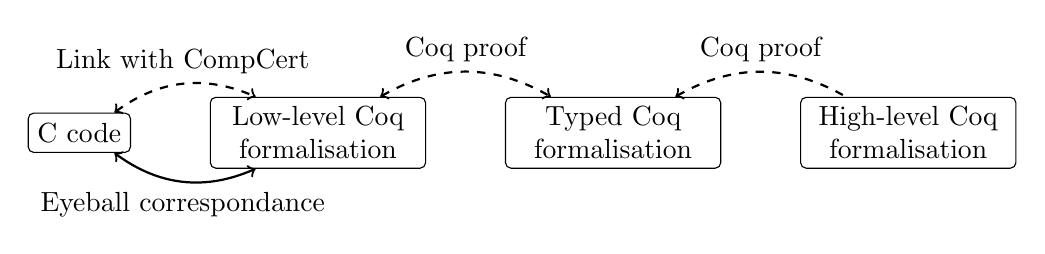
\begin{tikzpicture}
    \node [box] (C) {\Cn{} code} ;
    \node [box, right = 1cm of C] (low) {\parbox{25mm}{\centering{}Low-level \Coq{} formalisation}} ;
    \node [box, right = 1cm of low] (typed) {\parbox{25mm}{\centering{}Typed \Coq{} formalisation}} ;
    \node [box, right = 1cm of typed] (intuition) {\parbox{25mm}{\centering{}High-level \Coq{} formalisation}} ;

    \draw [<->, thick, dashed] (C) to [bend left] node [above] {Link with CompCert} (low) ;
    \draw [<->, thick] (low) to [bend left] node [below] {Eyeball correspondance} (C) ;
    \draw [<->, thick, dashed] (low) to [bend left] node [above] {\Coq{} proof} (typed) ;
    \draw [<-, thick, dashed] (typed) to [bend left] node [above] {\Coq{} proof} (intuition) ;
\end{tikzpicture}
\end{center}
At one end of the refinements is the \Cn{} source code of the \R{} interpreter.
As \R{} is defined by implementation,
this can be seen as a specification.
We in particular focus on the parts defining program evaluation
(mostly the files \texttt{src/include/Internal.h} and \texttt{src/main/eval.c}),
ignoring most constructs of the \R{} programming language.
A \Coq{} version of these \Cn{} definitions is defined,
with the aim to be the closest possible to the \Cn{} definition.
Some parts of the functions are dropped at this level,
such as error management.
At term, it is planned to use CompCert to prove that the \Coq{}
version is indeed identical to the chosen parts of the \Cn{} definition.

A typed \Coq{} formalisation is then defined.
This formalisation abstracts some low-level constructs,
such as pointers to basic language element
(which are heavily used in \R{}’s source code).
The expressions are also given a proper inductive at this stage,
although it is only weakly typed.
This inductive merely emphases with flag uses which pointers
of the basic language element structure.
It also makes explicit a subtlety of \Cn{} pointers,
which can be used for two distinct usages:
a pointer to one object,
or a pointer to an array of this object.
In this typed structure, the pointers to arrays
are replaced by a list,
which is much easier to manipulate in \Coq{}.

The last step of the process aims to fit
the intuition that the original had in mind when defining
the \R{} programming language~\parencite{ihaka1996r}.
Some advanced \R{} constructs may not fit such a high-level formalisation,
as they might break the underlying assumptions.


\subsection{Application}

Once a solid \Coq{} formalisation will be finished,
we aim to apply it by proving some properties on a \R{} program.
%
The \Coq{} formalisation does not contain any \R{} construct.
The first step will thus be to identify which constructs
are crucial for the analysis of the targeted program,
then provide them a specification
(either from the source, or a high-level one, which will have
to be tested against \R{}~\parencite{maj2013testr}).


\printbibliography

\end{document}

